\documentclass[border=10pt]{standalone}
\usepackage[left=25mm,right=25mm,top=25mm,bottom=25mm]{geometry}
\usepackage[utf8]{inputenc}
\usepackage[T1]{fontenc}
\usepackage{times}
\usepackage{geometry}
\usepackage{amsmath}
\usepackage{amssymb}
\usepackage{mathrsfs}
\usepackage{amsfonts}
\usepackage{amsthm}
\usepackage{lipsum}
\usepackage{amscd}
\usepackage{graphicx}
\usepackage{fancyhdr}
\usepackage{textcomp}
\usepackage{pgfplots}
\usepackage{txfonts}
\usepackage[all]{xy}
\usepackage{paralist}
\usepackage[colorlinks=true]{hyperref}
\usepackage{array}
\usepackage{tikz}
\usepackage{slashed}
\usepackage{pdfpages}
\usepackage{cite}
\usepackage{url}
\usepackage{amsmath,amsfonts,amssymb}
\usepackage{tikz}
\usetikzlibrary{arrows,matrix,positioning}
\usetikzlibrary{overlay-beamer-styles}
\usetikzlibrary{matrix.skeleton}
\usetikzlibrary{automata,positioning}
\usetikzlibrary{decorations.text}
\usepackage{listings}
\usepackage{multirow}
\usepackage{color}

\begin{document}

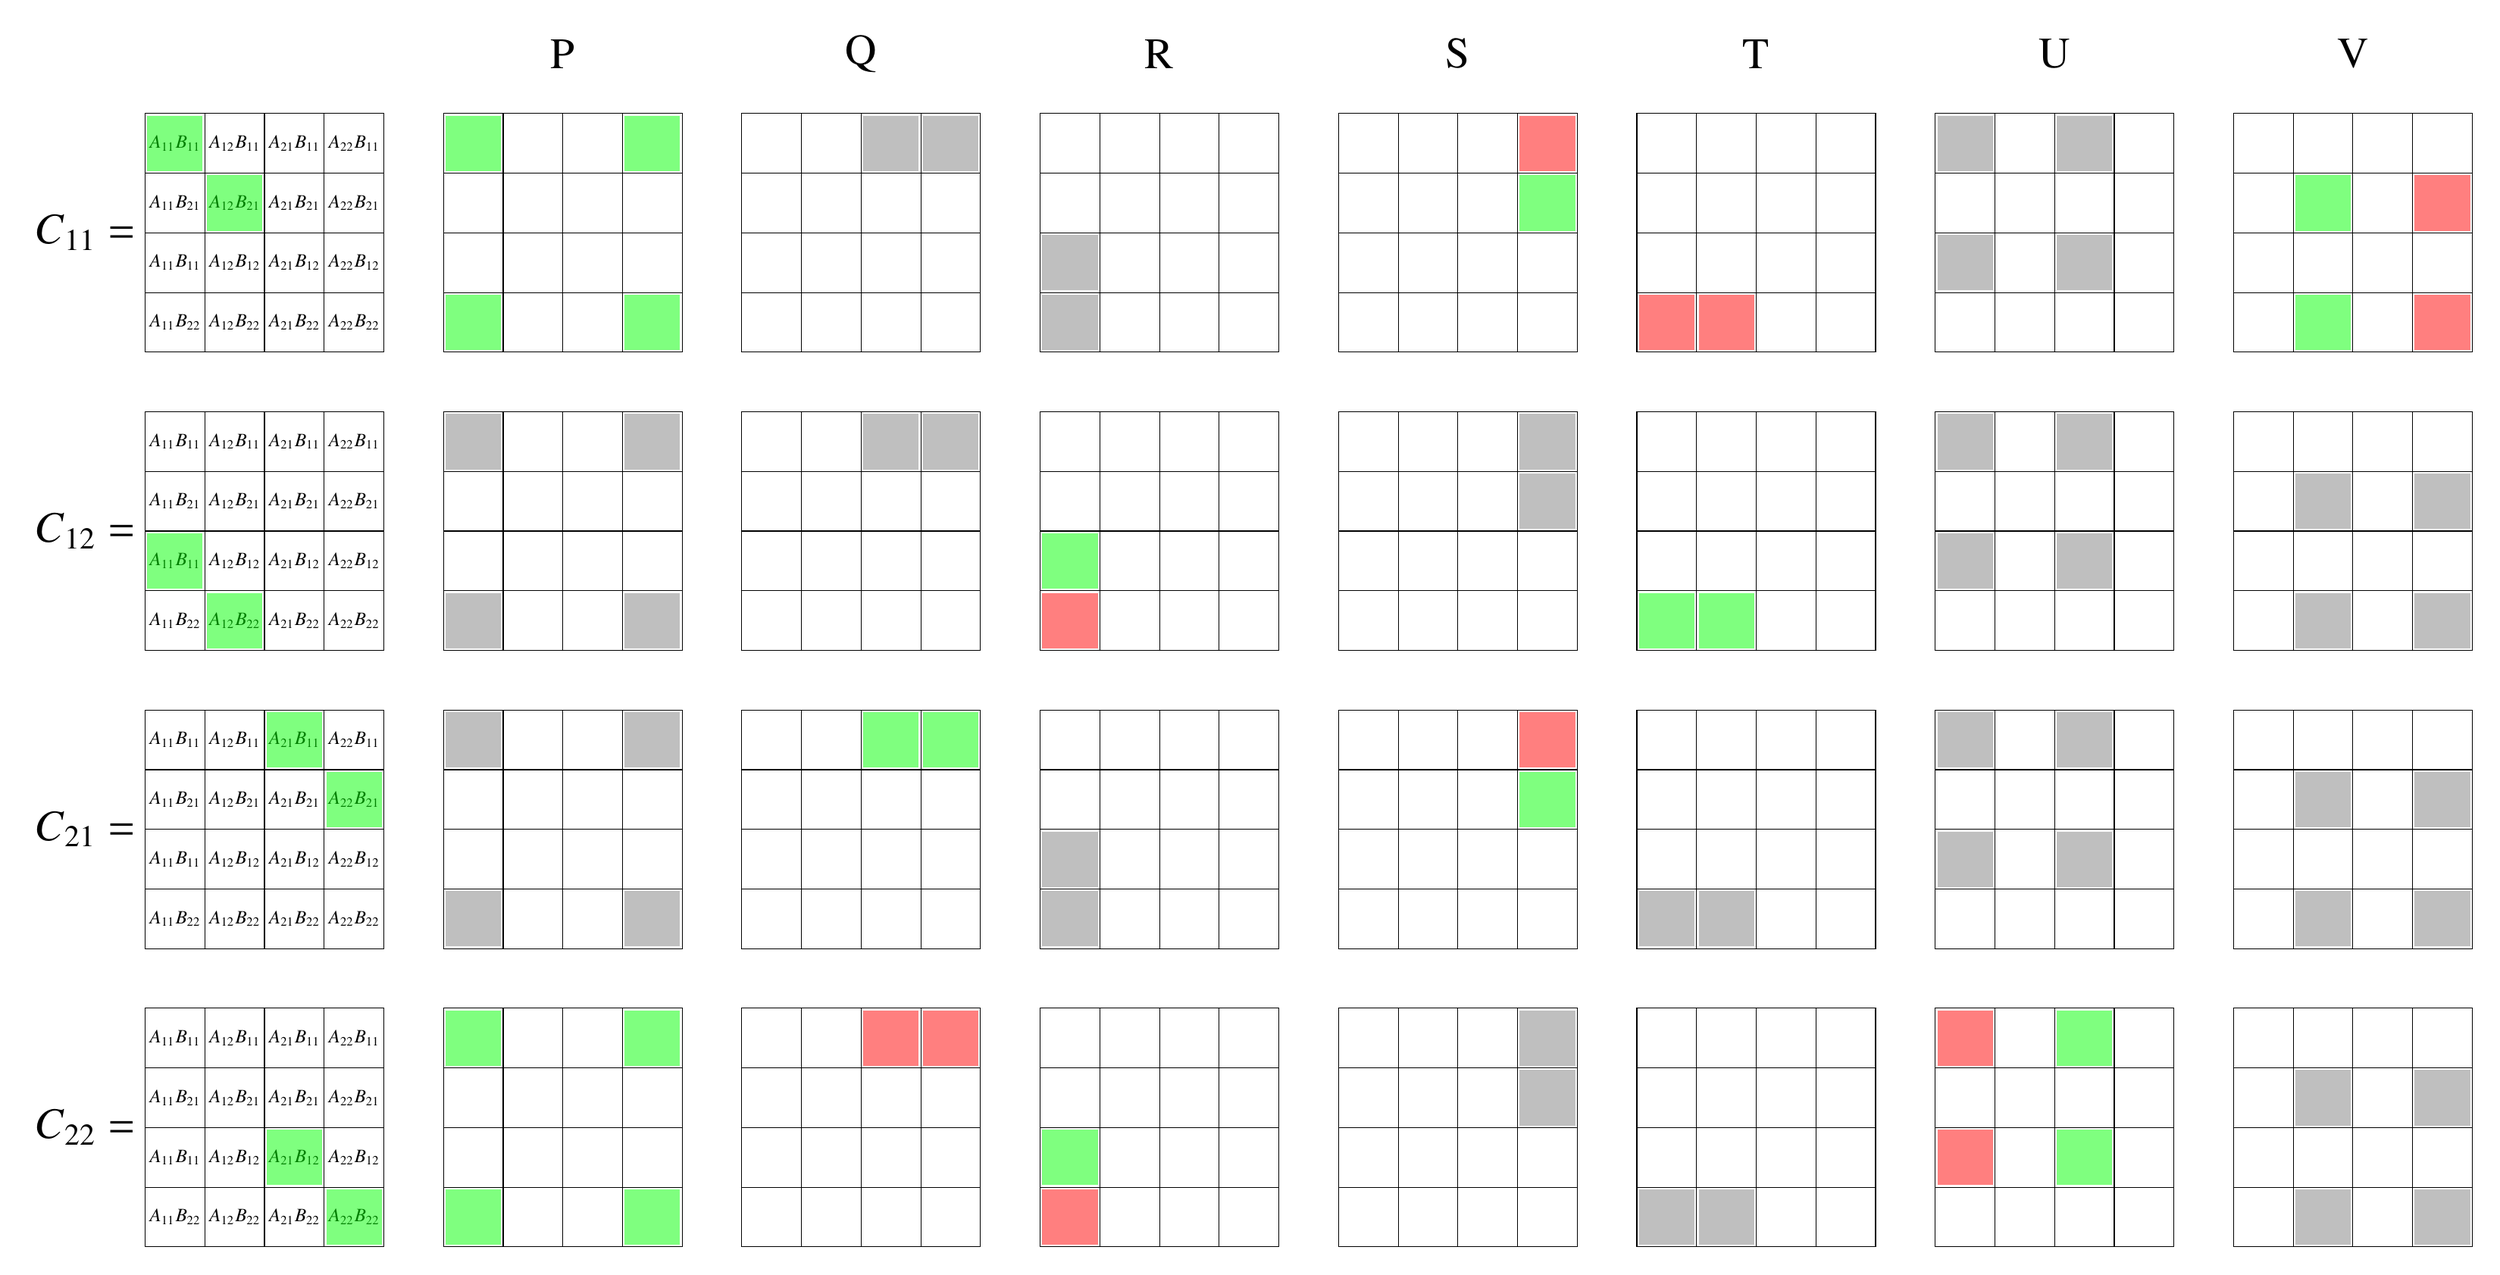
\begin{tikzpicture}[ampersand replacement=\&]

\foreach \i in {1,...,4}
{
	\small{
		\matrix (X\i)[matrix of math nodes,nodes in empty cells,
		nodes = {draw, minimum size=10mm,
			anchor=center,
			inner sep=0pt, outer sep=0pt},
		column sep=-\pgflinewidth,
		row sep=-\pgflinewidth,
		] at (0,-\i*5)
		{
			A_{11}B_{11} \& A_{12}B_{11} \& A_{21}B_{11} \& A_{22}B_{11} \\
			A_{11}B_{21} \& A_{12}B_{21} \& A_{21}B_{21} \& A_{22}B_{21} \\
			A_{11}B_{11} \& A_{12}B_{12} \& A_{21}B_{12} \& A_{22}B_{12} \\
			A_{11}B_{22} \& A_{12}B_{22} \& A_{21}B_{22} \& A_{22}B_{22} \\
		};}

	\foreach \j in {1,...,7}
	{
		\matrix(M\i\j)[matrix of math nodes,nodes in empty cells,
		nodes = {draw, minimum size=10mm,
			anchor=center,
			inner sep=0pt, outer sep=0pt},
		column sep=-\pgflinewidth,
		row sep=-\pgflinewidth,
		] at (\j*5,-\i*5)
		{
			\& \& \& \\
			\& \& \& \\
			\& \& \& \\
			\& \& \& \\
		};
	}
}

\huge{
	\node at (-3,-20)  {$C_{22}=$};
	\node at (-3,-15) {$C_{21}=$} ;
	\node at (-3,-10) {$C_{12}=$} ;
	\node at (-3,-5) {$C_{11}=$} ;

	\node at (5,-2)  {P};
	\node at (10,-2)  {Q};
	\node at (15,-2)  {R};
	\node at (20,-2)  {S};
	\node at (25,-2)  {T};
	\node at (30,-2)  {U};
	\node at (35,-2)  {V};
}


\node[opacity=0.5, rounded corners=0pt, inner sep=-1pt, fill=green, fit=(X1-1-1)] {};
\node[opacity=0.5, rounded corners=0pt, inner sep=-1pt, fill=green, fit=(X1-2-2)] {};
\node[opacity=0.5, rounded corners=0pt, inner sep=-1pt, fill=green, fit=(X2-3-1)] {};
\node[opacity=0.5, rounded corners=0pt, inner sep=-1pt, fill=green, fit=(X2-4-2)] {};
\node[opacity=0.5, rounded corners=0pt, inner sep=-1pt, fill=green, fit=(X3-1-3)] {};
\node[opacity=0.5, rounded corners=0pt, inner sep=-1pt, fill=green, fit=(X3-2-4)] {};
\node[opacity=0.5, rounded corners=0pt, inner sep=-1pt, fill=green, fit=(X4-3-3)] {};
\node[opacity=0.5, rounded corners=0pt, inner sep=-1pt, fill=green, fit=(X4-4-4)] {};

% P
\node[opacity=0.5, rounded corners=0pt, inner sep=-1pt, fill=green, fit=(M11-4-1)] {};
\node[opacity=0.5, rounded corners=0pt, inner sep=-1pt, fill=green, fit=(M11-1-4)] {};
\node[opacity=0.5, rounded corners=0pt, inner sep=-1pt, fill=green, fit=(M11-4-4)] {};
\node[opacity=0.5, rounded corners=0pt, inner sep=-1pt, fill=green, fit=(M11-1-1)] {};

\node[opacity=0.5, rounded corners=0pt, inner sep=-1pt, fill=gray, fit=(M21-4-1)] {};
\node[opacity=0.5, rounded corners=0pt, inner sep=-1pt, fill=gray, fit=(M21-1-4)] {};
\node[opacity=0.5, rounded corners=0pt, inner sep=-1pt, fill=gray, fit=(M21-4-4)] {};
\node[opacity=0.5, rounded corners=0pt, inner sep=-1pt, fill=gray, fit=(M21-1-1)] {};

\node[opacity=0.5, rounded corners=0pt, inner sep=-1pt, fill=gray, fit=(M31-4-1)] {};
\node[opacity=0.5, rounded corners=0pt, inner sep=-1pt, fill=gray, fit=(M31-1-4)] {};
\node[opacity=0.5, rounded corners=0pt, inner sep=-1pt, fill=gray, fit=(M31-4-4)] {};
\node[opacity=0.5, rounded corners=0pt, inner sep=-1pt, fill=gray, fit=(M31-1-1)] {};

\node[opacity=0.5, rounded corners=0pt, inner sep=-1pt, fill=green, fit=(M41-4-1)] {};
\node[opacity=0.5, rounded corners=0pt, inner sep=-1pt, fill=green, fit=(M41-1-4)] {};
\node[opacity=0.5, rounded corners=0pt, inner sep=-1pt, fill=green, fit=(M41-4-4)] {};
\node[opacity=0.5, rounded corners=0pt, inner sep=-1pt, fill=green, fit=(M41-1-1)] {};

% Q
\node[opacity=0.5, rounded corners=0pt, inner sep=-1pt, fill=gray, fit=(M12-1-4)] {};
\node[opacity=0.5, rounded corners=0pt, inner sep=-1pt, fill=gray, fit=(M12-1-3)] {};

\node[opacity=0.5, rounded corners=0pt, inner sep=-1pt, fill=gray, fit=(M22-1-4)] {};
\node[opacity=0.5, rounded corners=0pt, inner sep=-1pt, fill=gray, fit=(M22-1-3)] {};

\node[opacity=0.5, rounded corners=0pt, inner sep=-1pt, fill=green, fit=(M32-1-4)] {};
\node[opacity=0.5, rounded corners=0pt, inner sep=-1pt, fill=green, fit=(M32-1-3)] {};

\node[opacity=0.5, rounded corners=0pt, inner sep=-1pt, fill=red, fit=(M42-1-4)] {};
\node[opacity=0.5, rounded corners=0pt, inner sep=-1pt, fill=red, fit=(M42-1-3)] {};

% R

\node[opacity=0.5, rounded corners=0pt, inner sep=-1pt, fill=gray, fit=(M13-3-1)] {};
\node[opacity=0.5, rounded corners=0pt, inner sep=-1pt, fill=gray, fit=(M13-4-1)] {};

\node[opacity=0.5, rounded corners=0pt, inner sep=-1pt, fill=green, fit=(M23-3-1)] {};
\node[opacity=0.5, rounded corners=0pt, inner sep=-1pt, fill=red, fit=(M23-4-1)] {};

\node[opacity=0.5, rounded corners=0pt, inner sep=-1pt, fill=gray, fit=(M33-3-1)] {};
\node[opacity=0.5, rounded corners=0pt, inner sep=-1pt, fill=gray, fit=(M33-4-1)] {};

\node[opacity=0.5, rounded corners=0pt, inner sep=-1pt, fill=green, fit=(M43-3-1)] {};
\node[opacity=0.5, rounded corners=0pt, inner sep=-1pt, fill=red, fit=(M43-4-1)] {};

% S

\node[opacity=0.5, rounded corners=0pt, inner sep=-1pt, fill=red, fit=(M14-1-4)] {};
\node[opacity=0.5, rounded corners=0pt, inner sep=-1pt, fill=green, fit=(M14-2-4)] {};


\node[opacity=0.5, rounded corners=0pt, inner sep=-1pt, fill=gray, fit=(M24-1-4)] {};
\node[opacity=0.5, rounded corners=0pt, inner sep=-1pt, fill=gray, fit=(M24-2-4)] {};

\node[opacity=0.5, rounded corners=0pt, inner sep=-1pt, fill=red, fit=(M34-1-4)] {};
\node[opacity=0.5, rounded corners=0pt, inner sep=-1pt, fill=green, fit=(M34-2-4)] {};

\node[opacity=0.5, rounded corners=0pt, inner sep=-1pt, fill=gray, fit=(M44-1-4)] {};
\node[opacity=0.5, rounded corners=0pt, inner sep=-1pt, fill=gray, fit=(M44-2-4)] {};

%T

\node[opacity=0.5, rounded corners=0pt, inner sep=-1pt, fill=red, fit=(M15-4-1)] {};
\node[opacity=0.5, rounded corners=0pt, inner sep=-1pt, fill=red, fit=(M15-4-2)] {};

\node[opacity=0.5, rounded corners=0pt, inner sep=-1pt, fill=green, fit=(M25-4-1)] {};
\node[opacity=0.5, rounded corners=0pt, inner sep=-1pt, fill=green, fit=(M25-4-2)] {};

\node[opacity=0.5, rounded corners=0pt, inner sep=-1pt, fill=gray, fit=(M35-4-1)] {};
\node[opacity=0.5, rounded corners=0pt, inner sep=-1pt, fill=gray, fit=(M35-4-2)] {};

\node[opacity=0.5, rounded corners=0pt, inner sep=-1pt, fill=gray, fit=(M45-4-1)] {};
\node[opacity=0.5, rounded corners=0pt, inner sep=-1pt, fill=gray, fit=(M45-4-2)] {};

% U

\node[opacity=0.5, rounded corners=0pt, inner sep=-1pt, fill=gray, fit=(M16-1-3)] {};
\node[opacity=0.5, rounded corners=0pt, inner sep=-1pt, fill=gray, fit=(M16-1-1)] {};
\node[opacity=0.5, rounded corners=0pt, inner sep=-1pt, fill=gray, fit=(M16-3-3)] {};
\node[opacity=0.5, rounded corners=0pt, inner sep=-1pt, fill=gray, fit=(M16-3-1)] {};

\node[opacity=0.5, rounded corners=0pt, inner sep=-1pt, fill=gray, fit=(M26-1-3)] {};
\node[opacity=0.5, rounded corners=0pt, inner sep=-1pt, fill=gray, fit=(M26-1-1)] {};
\node[opacity=0.5, rounded corners=0pt, inner sep=-1pt, fill=gray, fit=(M26-3-3)] {};
\node[opacity=0.5, rounded corners=0pt, inner sep=-1pt, fill=gray, fit=(M26-3-1)] {};

\node[opacity=0.5, rounded corners=0pt, inner sep=-1pt, fill=gray, fit=(M36-1-3)] {};
\node[opacity=0.5, rounded corners=0pt, inner sep=-1pt, fill=gray, fit=(M36-1-1)] {};
\node[opacity=0.5, rounded corners=0pt, inner sep=-1pt, fill=gray, fit=(M36-3-3)] {};
\node[opacity=0.5, rounded corners=0pt, inner sep=-1pt, fill=gray, fit=(M36-3-1)] {};

\node[opacity=0.5, rounded corners=0pt, inner sep=-1pt, fill=green, fit=(M46-1-3)] {};
\node[opacity=0.5, rounded corners=0pt, inner sep=-1pt, fill=red, fit=(M46-1-1)] {};
\node[opacity=0.5, rounded corners=0pt, inner sep=-1pt, fill=green, fit=(M46-3-3)] {};
\node[opacity=0.5, rounded corners=0pt, inner sep=-1pt, fill=red, fit=(M46-3-1)] {};

%V

\node[opacity=0.5, rounded corners=0pt, inner sep=-1pt, fill=red, fit=(M17-2-4)] {};
\node[opacity=0.5, rounded corners=0pt, inner sep=-1pt, fill=red, fit=(M17-4-4)] {};
\node[opacity=0.5, rounded corners=0pt, inner sep=-1pt, fill=green, fit=(M17-2-2)] {};
\node[opacity=0.5, rounded corners=0pt, inner sep=-1pt, fill=green, fit=(M17-4-2)] {};


\node[opacity=0.5, rounded corners=0pt, inner sep=-1pt, fill=gray, fit=(M27-2-4)] {};
\node[opacity=0.5, rounded corners=0pt, inner sep=-1pt, fill=gray, fit=(M27-4-4)] {};
\node[opacity=0.5, rounded corners=0pt, inner sep=-1pt, fill=gray, fit=(M27-2-2)] {};
\node[opacity=0.5, rounded corners=0pt, inner sep=-1pt, fill=gray, fit=(M27-4-2)] {};

\node[opacity=0.5, rounded corners=0pt, inner sep=-1pt, fill=gray, fit=(M37-2-4)] {};
\node[opacity=0.5, rounded corners=0pt, inner sep=-1pt, fill=gray, fit=(M37-4-4)] {};
\node[opacity=0.5, rounded corners=0pt, inner sep=-1pt, fill=gray, fit=(M37-2-2)] {};
\node[opacity=0.5, rounded corners=0pt, inner sep=-1pt, fill=gray, fit=(M37-4-2)] {};

\node[opacity=0.5, rounded corners=0pt, inner sep=-1pt, fill=gray, fit=(M47-2-4)] {};
\node[opacity=0.5, rounded corners=0pt, inner sep=-1pt, fill=gray, fit=(M47-4-4)] {};
\node[opacity=0.5, rounded corners=0pt, inner sep=-1pt, fill=gray, fit=(M47-2-2)] {};
\node[opacity=0.5, rounded corners=0pt, inner sep=-1pt, fill=gray, fit=(M47-4-2)] {};





\end{tikzpicture}

\end{document}
